\documentclass[12pt]{article}
\usepackage[hmargin=1.25in, vmargin=1.1in]{geometry}

\usepackage[utf8]{inputenc}
\usepackage[T1]{fontenc}
\usepackage[francais]{babel}

\usepackage{listings}
\usepackage{color}
\usepackage{graphicx}
\usepackage{float}
\usepackage{upquote}
\usepackage{lastpage}
\usepackage{fancyhdr}
\pagestyle{fancy}
\usepackage{longtable}
\usepackage{tabu}

\graphicspath{ {images/} }

\newcommand{\helv}{\fontfamily{phv}\fontseries{b}\fontsize{9}{11}\selectfont}



%--------------- Variables à modifier à chaque rendu ---------------
\title{Rendu 1}
\newcommand{\daterendu}{12/10/2017}
%-------------------------------------------------------------------

\makeatletter\let\Title\@title\makeatother

% Décommenter pour commencer les chapitres à 0
%\setcounter{section}{-1}

\begin{document}

\begin{titlepage}

\newcommand{\HRule}{\rule{\linewidth}{0.5mm}} % Defines a new command for the horizontal lines, change thickness here

\center % Center everything on the page



\includegraphics[width=\textwidth]{logo_HEIA.jpg}\\[1.3cm]
\textsc{\Large Génie Logiciel 2 \\ [0.4cm]
\large Automne 2016-2017 \\ [0.4cm]
\large Mini-Projet SimuLife}\\[1.8cm] 


\textsc{
\bfseries \LARGE Water World\\ [0.8cm]
\Large Groupe No : 6}\\[1.4cm]


\HRule \\[0.4cm]
{ \huge \bfseries \Title }\\ 
\HRule \\[1.2cm]

\Large 
Bastien \textsc{Monney}\\[0cm]
Nicolas \textsc{Fuchs}\\[0cm]
Guillaume \textsc{Michel}\\[1.7cm] 

{\large Date du rendu : \daterendu}\\[1.5cm] 

\begin{center}
\large Enseignant : Pierre Kuonen / Julien Tscherrig
\end{center}

\end{titlepage}
\pagenumbering{Roman}

\renewcommand{\headrulewidth}{1pt}
\fancyhead[L]{\helv WaterWorld}
\fancyhead[C]{\helv 2017-2018}
\fancyhead[R]{\helv \Title }

\renewcommand{\footrulewidth}{1pt}
\fancyfoot[C]{\helv Table des matières \thepage{}}

\setcounter{page}{1}

\begin{center}
\renewcommand{\contentsname}{Table des matières}
\tableofcontents
\end{center}

\newpage
 {\setlength{\baselineskip}{1.5\baselineskip}
\fancyhf{}
\renewcommand{\headrulewidth}{1pt}
\fancyhead[L]{\helv Nom du Groupe}
\fancyhead[C]{\helv 2016-2017}
\fancyhead[R]{\helv \Title }

\renewcommand{\footrulewidth}{1pt}
\fancyfoot[L]{\helv GL2-Info, Automne 2017 - 2018}
\fancyfoot[C]{}
\fancyfoot[R]{\helv \textbf{Page \thepage{} sur \pageref{LastPage}}}
\pagenumbering{arabic}
\setcounter{page}{1}
\section{Les créatures du monde:}
\begin{itemize}
	\item Une Orque unique
	\item Des requins
	\item Des pingouins
	\item De la banquise
\end{itemize}
\section{Règles du jeu:}
	L'orque:
	\begin{itemize}
		\item Mouvements aléatoires
		\item Un déplacement par tour
		\item Déplacement aléatoire sans foncer dans un élément
		\item Reste dans l'eau et n'a pas besoin de se nourrir
	\end{itemize}	
	Les requins:
	\begin{itemize}
		\item Sentent les pingouins dans l'eau et essaient d'aller manger le plus proche. (donc ils connaissent la position du pingouin le plus proche d'eux qui se situe dans l'eau)
		\item S'ils ne "sentent" aucun pingouin, ils se déplacent aléatoirement
		\item Un déplacement par tour
		\item S'ils ne mangent pas, ils meurent au bout de 10 tours. Chaque "nourriture" rajoute 10 tours "de vie" au requin.
		\item Pour manger, un requin doit se trouver sur la même case qu'un pingouin.
		\item Ils ne peuvent pas aller sur la banquise.
	\end{itemize}
\newpage
	Les pingouins:
	\begin{itemize}
		\item Se déplacent d'une case un tour sur deux.
		\item Par défaut se déplacent aléatoirement.
		\item Repèrent les requins se trouvant à 2 cases d'eux (et 1 case en diagonale)
		\item S'ils voient un requin, le fuient vers la banquise si possible sinon dans le sens opposé au requin (si possible sinon random)
		\item une fois sur la banquise, le pingouin est en sécurité
		\item descendent de la banquise dès qu'il y a possibilité de descendre (donc aucun requin du côté de la banquise ou le pingouin veut descendre)
	\end{itemize}
	La banquise:
	\begin{itemize}
		\item A chaque tour, aléatoirement, on choisit si oui ou non on modifie la banquise (pour chaque élément de la banquise) puis si elle doit réduire ou grandire. Ensuite on l'aggrandi ou rétrécie de 1 case d'après l'espace disponible. Dès qu'il ne reste qu'une case, la banquise disparaît complètement et met le pingouin à l'eau s'il y en avait un dessus.
	\end{itemize}

	Général:
	\begin{itemize}
		\item Les déplacements se font d'une case à la fois et seulement par les côtés, pas en diagonale.
		\item Le jeu s'arrête dès que tous les requins sont morts ou alors dès que tous les pingouins ont été mangés.
	\end{itemize}
	\medskip
	Champs de vision d'un pingouin: \\
	\begin{center}
		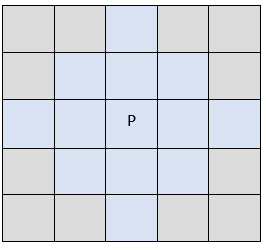
\includegraphics[width=5cm]{schema_Pingouin.png}\\[0.3cm]
	\end{center}
\newpage
\section{Diagramme d'activités}

			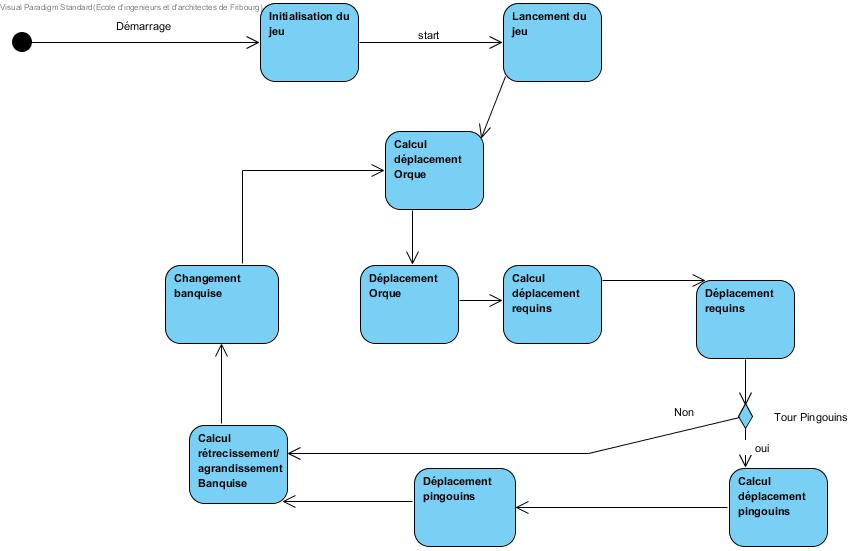
\includegraphics[width=15cm]{WaterWorld.jpg}\\[0.3cm]
\end{document}